\documentclass[11pt]{article}
\usepackage[utf8]{inputenc}
\usepackage[T1]{fontenc}
\usepackage[margin=1in]{geometry}
\usepackage{amsmath,amssymb,amsthm,booktabs,longtable,hyperref,fancyvrb}
\usepackage{tikz}
\usetikzlibrary{arrows.meta,positioning}
\newtheorem{theorem}{Theorem}
\newtheorem{lemma}[theorem]{Lemma}
\newtheorem{proposition}[theorem]{Proposition}
\newtheorem{corollary}[theorem]{Corollary}
\theoremstyle{remark}
\newtheorem{remark}[theorem]{Remark}
\newcommand{\ML}{\mathrm{ML}}
\newcommand{\R}{\mathbb{R}}
\newcommand{\Z}{\mathbb{Z}}
\newcommand{\Q}{\mathbb{Q}}
\newcommand{\dist}[1]{\lVert #1\rVert}
\ExplSyntaxOn
\NewDocumentCommand{\lean}{m}
 {%
  {\small\texttt{%
   \tl_set:Nx \l_tmpa_tl { \detokenize{#1} }
   \tl_replace_all:Nnn \l_tmpa_tl { . } { .\allowbreak }
   \tl_replace_all:Nnn \l_tmpa_tl { / } { /\allowbreak }
   \exp_args:NNxx \tl_replace_all:Nnn \l_tmpa_tl
    { \c_underscore_str } { \c_underscore_str \exp_not:N \allowbreak }
   \tl_use:N \l_tmpa_tl
  }}%
 }
\ExplSyntaxOff
\setlength{\emergencystretch}{3em}
% Unicode glyphs occurring in the verbatim copies of the Lean statements (the text of the files is not altered)
\DeclareUnicodeCharacter{2124}{\ensuremath{\mathbb Z}}
\DeclareUnicodeCharacter{211D}{\ensuremath{\mathbb R}}
\DeclareUnicodeCharacter{2115}{\ensuremath{\mathbb N}}
\DeclareUnicodeCharacter{2200}{\ensuremath{\forall}}
\DeclareUnicodeCharacter{2203}{\ensuremath{\exists}}
\DeclareUnicodeCharacter{2208}{\ensuremath{\in}}
\DeclareUnicodeCharacter{2227}{\ensuremath{\wedge}}
\DeclareUnicodeCharacter{2264}{\ensuremath{\leq}}
\DeclareUnicodeCharacter{2192}{\ensuremath{\to}}
\DeclareUnicodeCharacter{00D7}{\ensuremath{\times}}
\DeclareUnicodeCharacter{03C4}{\ensuremath{\tau}}
\title{The lonely runner conjecture for eight and nine runners:\\ a kernel-checked proof}
\author{Vico Bonfioli}
\date{19 November 2026}
\begin{document}
\maketitle

\begin{abstract}
For positive integer speeds $v_1,\dots,v_n$ let $\ML(v)=\max_t\min_i\dist{tv_i}$, where $\dist{x}$ is the distance from $x$ to the nearest integer. The lonely runner conjecture for $n+1$ runners asserts $\ML(v)\ge1/(n+1)$. We prove it in Lean~4, against Mathlib, for eight runners (seven speeds) and for nine runners (eight speeds), with no hypothesis and with no axiom beyond the three standard ones of Lean. The proof follows the computer-assisted reductions of Rosenfeld and of Trakulthongchai. For eight runners the reduction needs a covering condition modulo $8p$ for each of $27$ primes $p$, together with the seven-runner theorem of Barajas and Serra, which is formalized as well. For nine runners it needs a covering condition modulo $p$, $3p$ and $9p$ for each of $36$ primes, established by cover trees with $33{,}384{,}638$ nodes in all, and it uses the eight-runner theorem as its only hypothesis. The finite parts are certificates generated by Rust programs and checked by the Lean kernel. The final theorem is assembled in one elaboration by the Lean compiler run directly on archived compiled files, which the build tool of the project does not track; we say precisely what that does and does not establish. Both statements were proved earlier on paper, with computer assistance, by Rosenfeld and by Trakulthongchai; the contribution here is the formal proof and the certificate method.
\end{abstract}

\section{Introduction}\label{sec:intro}

For a vector $v=(v_1,\dots,v_n)$ of positive integers put
\[
\ML(v)=\max_{t\in\R}\ \min_{1\le i\le n}\dist{tv_i},\qquad \dist{x}=\min(\{x\},1-\{x\}).
\]
Think of $n+1$ runners on a circular track of length one, one of them standing still and the others running with the constant speeds $v_i$; $\ML(v)$ is the largest distance from the stationary runner that can be achieved at one time simultaneously from all the others. The lonely runner conjecture of Wills~\cite{Wills} and of Cusick~\cite{Cusick} states that $\ML(v)\ge1/(n+1)$ for all $n$ and all positive integer speeds. Write $\mathrm{LRC}(n)$ for the statement ``$\ML(v)\ge 1/(n+1)$ for every $v\in\Z^n$ with positive entries''. Throughout, \emph{the number of runners is the number of speeds plus one}. The statement $\mathrm{LRC}(n)$ is known for $n\le 6$ by the work of Cusick and Pomerance~\cite{CP}, Bohman, Holzman and Kleitman~\cite{BHK}, Renault, and Barajas and Serra~\cite{BS}; Rosenfeld~\cite{Ros8} proved $\mathrm{LRC}(7)$ (eight runners) by a computer-assisted argument and later~\cite{Ros9} $\mathrm{LRC}(8)$ (nine runners); Trakulthongchai~\cite{Tra} obtained nine and ten runners by refining the method with a sieve, and Sungkawichai and Trakulthongchai~\cite{ST} reached eleven, twelve and thirteen runners.

We prove the two statements $\mathrm{LRC}(7)$ and $\mathrm{LRC}(8)$ in Lean~4 with Mathlib.

\begin{theorem}[eight runners]\label{thm:eight}
For every $v\in\Z^7$ with positive entries, $\ML(v)\ge 1/8$. (Lean: \lean{LRSpectrumFull.EightRunnersReal.eight_runners_unconditional_real}.)
\end{theorem}

\begin{theorem}[nine runners]\label{thm:main}
For every $v\in\Z^8$ with positive entries, $\ML(v)\ge 1/9$. (Lean: \lean{LRSpectrumFull.NineSound.Plan9.Assemble9Final.nine_runners_unconditional}.)
\end{theorem}
Both formal statements have no hypothesis other than positivity of the speeds, and the output of \texttt{\#print axioms} for each is exactly \lean{propext}, \lean{Classical.choice}, \lean{Quot.sound}. The statements are listed verbatim in Section~\ref{sec:lean}.

\paragraph{The chain.} Theorem~\ref{thm:eight} is derived from (i) $\mathrm{LRC}(6)$, the seven-runner theorem of Barajas and Serra, which is formalized in the same development; (ii) the reduction of Rosenfeld, formalized, which says that in a counterexample the product of the speeds is divisible by $840\prod_{p\in S_7}p$ for a set $S_7$ of $27$ primes; and (iii) $27$ finite checks, one per prime, each proved by kernel evaluation of a generated certificate (Section~\ref{sec:eight}). Theorem~\ref{thm:main} is derived from Theorem~\ref{thm:eight} used as the hypothesis $\mathrm{LRC}(7)$, from the analogous reduction at nine runners, and from $36$ finite checks of cover trees (Sections~\ref{sec:red}--\ref{sec:cert}). The final assembly is the module \lean{Assemble9Final}, which proves $\mathrm{LRC}(7)$ from Theorem~\ref{thm:eight} (a numeral conversion $1/((6:\R)+2)=1/8$) and feeds it to the nine-runner theorem that takes $\mathrm{LRC}(7)$ as an explicit argument. Which parts of this chain are tracked by the build tool of the project and which were assembled by the compiler run directly is stated in Section~\ref{sec:trust}; it matters for how much weight the word ``kernel-checked'' carries.

\paragraph{What is new and what is not.} Both mathematical statements are not new. Rosenfeld~\cite{Ros8,Ros9} and Trakulthongchai~\cite{Tra} proved them by computer-assisted arguments (their code is in C++ and Python; no formalization of them is known to us). The reductions we follow are theirs, resting on the finite-checking theorem of Malikiosis, Santos and Schymura~\cite{MSS}: the prime-divisibility criterion, the product bound, the use of rational times with denominator $(k+1)p$ and the lifting to multiples of $p$ are in~\cite{Ros8,Tra,ST}. What we claim is (i) formal proofs, in Lean~4 and Mathlib, of $\mathrm{LRC}(7)$ and $\mathrm{LRC}(8)$ with only the standard axioms, including a formal proof of $\mathrm{LRC}(6)$ and a replacement of the height bound of~\cite{MSS} by a pigeonhole lemma and the rounding step of Giri and Kravitz~\cite{GK}; (ii) the certificates, in the form of kernel-checked searches for $27$ and, as cover trees, for $36$ primes, together with the soundness proofs of the checkers; (iii) an explicit choice of the $36$ primes by a knapsack on the size of the certificates; and (iv) the engineering that makes a $33$-million-node certificate checkable in a proof assistant on one workstation. We do not claim a new proof of either statement, and, as nothing in our records is a search for formalizations of these two statements, we make no claim of priority for a formal proof (Section~\ref{sec:prior}).

\paragraph{Contents.} Section~\ref{sec:eight} treats eight runners. Section~\ref{sec:red} proves the nine-runner reduction on paper, up to the finite condition on each prime. Section~\ref{sec:cover} states the finite condition and the cover tree that establishes it, and explains the choice of primes. Section~\ref{sec:cert} describes the certificates and how the kernel checks them. Section~\ref{sec:lean} gives the formal statements. Section~\ref{sec:trust} lists the trust base and what is and is not verified. Section~\ref{sec:meas} gives measurements. Sections~\ref{sec:limits}, \ref{sec:repro}, \ref{sec:prior} and~\ref{sec:prov} contain limitations, reproducibility, prior art and provenance.

\section{Eight runners}\label{sec:eight}

\subsection{The finite check}\label{sec:l7}

Both theorems rest on one Boolean function, which we state for general $k$ (the number of speeds). Let $q=(k+1)p$ for a prime $p>k+1$, let $W=\{1,\dots,\lfloor q/2\rfloor\}$ and let $A=\{x\in W:p\nmid x\}$. For $x\in A$ and $j\in W$ say that \emph{$x$ covers $j$} if $\dist{jx/q}<1/(k+1)$, that is, if $(k+1)\min(r,q-r)<q$ with $r=jx\bmod q$. A $k$-element subset $V\subseteq A$ is \emph{admissible} if for every prime $\ell\mid k+1$ at most $k-2$ elements of $V$ are divisible by $\ell$. Then
\[
\texttt{lemma7Check}(k,p)=\texttt{true}\iff\text{no admissible $V\subseteq A$ of size $k$ covers $W$},
\]
that is, for no admissible $V$ does every $j\in W$ have an $x\in V$ covering it. In Lean this is the following definition (module \lean{LRCFourRunnersCore}; the auxiliary definitions \lean{coversAt}, \lean{admissible}, \lean{sideOK}, \lean{coversWindow} and \lean{tuples} are in the same file and are exactly the prose above).
\VerbatimInput[fontsize=\footnotesize,frame=single,framesep=2mm,label={lemma7Check (LRCFourRunnersCore)}]{snippets/l7check_def.lean}
For $k=7$ the only prime dividing $k+1=8$ is $2$: at most five of the seven elements are even, and the modulus is $8p$. For $k=8$ the only prime dividing $9$ is $3$: at most six of the eight elements are multiples of $3$, and the modulus is $9p$. The side condition is stated as a divisibility count, which is the form that the leave-one-out step of Rosenfeld's argument delivers (Lemma~\ref{lem:three} below, and its analogue for $k=7$).

\subsection{Rosenfeld's reduction at seven speeds}\label{sec:ros7}

Lean names in this subsection are in the namespace \lean{LRSpectrumFull.EightPlan} unless stated otherwise. A counterexample is a primitive $v\in\Z^7$ with positive entries and $\ML(v)<1/8$. Since $\ML(cv)=\ML(v)$ for every integer $c\neq0$, a counterexample exists iff one exists among all positive vectors (\lean{e0_primitive}). The steps, for a counterexample $v$ and assuming $\mathrm{LRC}(6)$, are as follows.
\begin{itemize}
\item (leave-one-out, \cite[Lemma~5]{Ros8}) Deleting any one speed leaves six speeds with greatest common divisor $1$; in particular at most five of the seven speeds are even (\lean{e4_leaveOneOut}, \lean{e4_parity}). The proof is the gcd lemma, Lemma~\ref{lem:gcd} below, at $k_0=5$.
\item (prime lemma, \cite[Lemmas~6,~7]{Ros8}) If \lean{lemma7Check 7 p = true}, then $p$ divides some speed of $v$ (\lean{e2_prime_dvd}). The argument is that of Lemma~\ref{lem:prime} below with $k=7$.
\item (small divisors) For each of $j=8,3,5,7$, some speed is divisible by $j$, otherwise the time $1/j$ gives $\ML(v)\ge 1/j\ge1/8$; so $840=8\cdot3\cdot5\cdot7$ divides $\prod v_i$. Together with the prime lemma, $840\prod_{p\in S_7}p$ divides $\prod v_i$ (\lean{e3_lcm_dvd}).
\item (arithmetic) $28^{42}<7^7\cdot840\prod_{p\in S_7}p$ (\lean{numeric}), and by the arithmetic--geometric mean inequality $28^{42}<7^7\prod v_i$ implies $\sum v_i>28^6$ (\lean{e5_amgm}).
\item (rounding) Assuming $\mathrm{LRC}(6)$, a primitive $v\in\Z^7$ with positive entries and $\sum v_i>28^6$ has $\ML(v)\ge1/8$ (\lean{EightE5.e5_sum}, \lean{EightE5.e5_prod}). This is Lemma~\ref{lem:round} with seven speeds in place of eight; it is obtained from the staircase lemma below and the rounding step, the latter with $28=7\cdot8/2$ in place of $36$ and the bound $1/7-1/56=1/8$ in place of $1/8-1/72=1/9$.
\end{itemize}
The set of primes is
\begin{quote}\small\raggedright$S_7=\{31,\allowbreak 37,\allowbreak 43,\allowbreak 47,\allowbreak 53,\allowbreak 59,\allowbreak 61,\allowbreak 67,\allowbreak 71,\allowbreak 73,\allowbreak 79,\allowbreak 83,\allowbreak 89,\allowbreak 97,\allowbreak 101,\allowbreak 103,\allowbreak 107,\allowbreak 109,\allowbreak 113,\allowbreak 127,\allowbreak 131,\allowbreak 137,\allowbreak 139,\allowbreak 149,\allowbreak 151,\allowbreak 157,\allowbreak 163\}$\end{quote}
the $27$ primes in $[31,163]$ other than $41$ (\lean{rosenfeldS}). The assembly of the steps is the theorem \lean{EightE5.eight_runners_of}, which takes $\mathrm{LRC}(6)$ and the $27$ statements \lean{lemma7Check 7 p = true} as hypotheses (the last line of the proof is cut):
\VerbatimInput[fontsize=\footnotesize,frame=single,framesep=2mm,label={eight\_runners\_of (EightE5)}]{snippets/eight_of.lean}
Its axiom print is the three standard axioms.

\begin{lemma}[staircase; Lean: \lean{EightMSS.e5b_staircase}, and the copy \lean{Stair9.e5b_staircase}]\label{lem:stair}
Let $v\in\Z^n$ be primitive with positive entries and let $l\ge1$ be an integer with $\sum_iv_i>l^{n-1}$. There are $z\in\Z^n$, not proportional to $v$, and $\sigma\in\Q$ with $|lz_i-\sigma v_i|\le1$ for all $i$.
\end{lemma}
\begin{proof}[Sketch]
For each pair $e=(i,a)$ with $0\le a<v_i$ put $\tau_e=(2a+1)/(2v_i)$ and let $q_e\in\Z^n$ be the coordinatewise rounding of $\tau_ev$, with ties broken by the index order, so that the $\sum_iv_i$ points $q_e$ are distinct and $|q_{e,j}-\tau_ev_j|\le1/2$. The map $(e,c)\mapsto q_e+cv\bmod l$ on pairs with $0\le c<l$ has $l\sum_iv_i>l^n$ arguments, so two collide. If they share $e$, primitivity gives $l\mid c-c'$, which is impossible. Otherwise $lz=q_e-q_{e'}-(c'-c)v$ defines $z\in\Z^n$, and $\sigma=\tau_e-\tau_{e'}-(c'-c)$ satisfies the bound. If $z$ were proportional to $v$, primitivity would give $q_e-q_{e'}=sv$ with $s\in\Z$, and the bounds $0\le q_{e,k}<v_k$ at the index $k$ of $e$ (and of $e'$) force $s=0$, contradicting $q_e\ne q_{e'}$.
\end{proof}
Rosenfeld obtains the corresponding height bound from a theorem of Malikiosis, Santos and Schymura~\cite{MSS} whose proof passes through zonotopes and successive minima; we did not formalize that proof. The pigeonhole lemma above and the planar rounding step of Giri and Kravitz~\cite{GK} (the case $r=1$ of~\cite[Proposition~3.4]{All}) take its place, with the same modulus $l=\binom{n+1}{2}$ and the same threshold $l^{n-1}$ as in~\cite{Ros8}.

\subsection{Seven runners}\label{sec:bs}

The hypothesis $\mathrm{LRC}(6)$ is the theorem of Barajas and Serra~\cite{BS}, formalized in the same development (\lean{BarajasSerra.LRC6_barajasSerra}, from \lean{BarajasSerra.Sec5.lrc6}); its axiom print is the three standard axioms, and it is part of the package built by \lean{lake}. The formalization follows the printed proof: a prime-filtering lemma by descending induction on the $p$-adic levels of the speeds, a case analysis by the distribution of the speeds over the levels, and, for the hardest configuration (five speeds at level $0$ and one above), a kernel-evaluated table modulo $98$ for $m=1$ and a pattern analysis of residues modulo $7$ for $m\ge2$. The three-runner and five-runner subcases that the printed proof does not settle by filtering are decided by finite models checked by the kernel. In the course of the formalization eleven places of the printed proof were found to need correction (wrong ranges, signs or intermediate values, one claim that is false as printed for two profiles but is not used, and one implication that fails in $28$ of $12{,}544$ model configurations although the claim it was meant to give is true); none affects the theorem, and each repair is local. We did not otherwise re-read this part for the present paper beyond its statement and axiom print.

\subsection{The $27$ certificates}\label{sec:eight-cert}

Evaluating \lean{lemma7Check 7 p} directly in the kernel is infeasible for the larger primes. A second checker, \lean{EightCheckV4}, walks a search tree supplied as data (a certificate) and accepts only if every leaf is closed by a counting bound or a table lookup. Its soundness theorem \lean{EightV4.lemma7Check_of_checkRootH} states that acceptance implies \lean{lemma7Check 7 p = true}, and its axiom print is the three standard axioms. A Rust program generates, for each prime, the certificate as Lean source split into modules (about $1.6$ GB in all for the $27$ primes); the kernel evaluates the checker on it by \lean{decide +kernel} (kernel evaluation of a Boolean expression, no native compilation). A wrong certificate is rejected by the checker and cannot give a false theorem; the generator is not in the trust base.

For each prime $p\in S_7$ the proof of \lean{lemma7Check 7 p = true} is the theorem \lean{EightV4.Cert}$p$\lean{.lemma7Check_seven_p}$p$, produced by a staged build, one Lean process per module, in modules \lean{E8Stage.P}$p$\lean{.*} whose last module \lean{Asm} proves the theorem. A record file per prime stores the generator command, the SHA-256 digest of the generator, of the checker, of the soundness file, of each generated module and of the concatenation of the modules, the toolchain, and the axiom print of the theorem. The staged compiled files of the $27$ primes (949 files, about $2.5$ GB) are kept outside the \lean{lake} package. Table~\ref{tab:eight} lists the kernel wall time of each prime in the original build: in all $38{,}567$ seconds ($10.7$ hours) of summed module time, between $36$ s and $5{,}286$ s per prime, and a largest recorded peak footprint of $1.08$ GB (at $p=163$). The module \lean{EightRunnersReal} imports the $27$ \lean{Asm} modules, restates the $27$ checks as one case split \lean{hchk_all_real}, and proves Theorem~\ref{thm:eight} by applying \lean{eight_runners_of} to \lean{BarajasSerra.LRC6_barajasSerra} and \lean{hchk_all_real}.

\begin{table}[ht]
\centering\small
\begin{tabular}{rrrrrrrrrrrr}
\toprule
$p$ & s & $p$ & s & $p$ & s & $p$ & s & $p$ & s & $p$ & s\\
\midrule
31 & 89 & 37 & 139 & 43 & 86 & 47 & 98 & 53 & 229 & 59 & 361\\
61 & 36$^\ast$ & 67 & 394 & 71 & 281 & 73 & 391 & 79 & 370 & 83 & 544\\
89 & 834 & 97 & 1082 & 101 & 1032 & 103 & 956 & 107 & 1267 & 109 & 1415\\
113 & 1796 & 127 & 1791 & 131 & 2369 & 137 & 3279 & 139 & 2959 & 149 & 3607\\
151 & 3409 & 157 & 4467 & 163 & 5286\\
\bottomrule
\end{tabular}
\caption{Kernel wall seconds per prime of the original staged build ($^\ast$: a resumed run, so not the full time).}\label{tab:eight}
\end{table}

\paragraph{History of this step.} In the default package build, the $27$ checks enter an earlier form of Theorem~\ref{thm:eight}, \lean{EightE5.eight_runners_unconditional}, as $27$ axioms \lean{EightCert27.lemma7Check_seven_p}$p$\lean{_verified}, each recording a kernel check that had been run and whose sources were then deleted to save disk space; the module \lean{EightE5} imports them. The theorem used here does not use these axioms: \lean{eight_runners_of} takes the checks as a hypothesis, and the print of the axioms of \lean{eight_runners_unconditional_real} lists only the three standard ones. The $27$ axioms are, however, present in the import closure of the module \lean{EightE5} and therefore in the environment in which the final theorem is elaborated; a reader who wants this to be beyond doubt should check the axiom print of the final theorem and not only the absence of the axioms from the text of the final modules. The certificates of all $27$ primes were regenerated at least once and their hashes matched the recorded ones.

\section{The reduction for nine runners}\label{sec:red}

Fix $k=8$ speeds. In this section $\mathrm{LRC}(7)$ is a hypothesis; Theorem~\ref{thm:eight} supplies it in the final assembly (Section~\ref{sec:lean}). A \emph{counterexample} is $v\in\Z^8$ with positive entries and $\ML(v)<1/9$; it is \emph{primitive} if $\gcd(v_1,\dots,v_8)=1$. Since $\ML(cv)=\ML(v)$ for every integer $c\ne0$, a counterexample exists iff a primitive one does. (The scaling argument is \lean{e0_primitive9}, the analogue of \lean{e0_primitive} of Section~\ref{sec:ros7}.) The map $v\mapsto\ML(v)$ is invariant under sign changes and permutations of the speeds.

The argument is the one of~\cite{Ros8,Tra} with the constants of $k=8$. Figure~\ref{fig:chain} shows the dependencies; the steps are proved in this section, except that the finite condition $C(p)$ of Section~\ref{sec:cover} is taken as given.

\begin{figure}[ht]
\centering
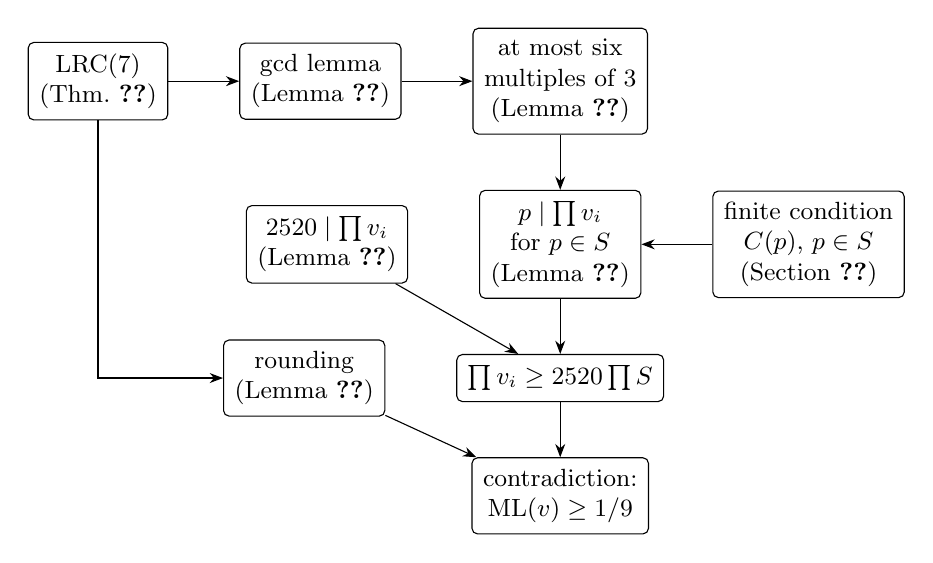
\begin{tikzpicture}[node distance=7mm and 9mm, every node/.style={font=\small}, box/.style={draw, rounded corners=2pt, align=center, inner sep=4pt}]
\node[box] (L7) {$\mathrm{LRC}(7)$\\ (Thm.~\ref{thm:eight})};
\node[box, right=of L7] (gcd) {gcd lemma\\ (Lemma~\ref{lem:gcd})};
\node[box, right=of gcd] (three) {at most six\\ multiples of $3$\\ (Lemma~\ref{lem:three})};
\node[box, below=of three] (prime) {$p\mid\prod v_i$\\ for $p\in S$\\ (Lemma~\ref{lem:prime})};
\node[box, left=of prime] (small) {$2520\mid\prod v_i$\\ (Lemma~\ref{lem:small})};
\node[box, below=of prime] (prod) {$\prod v_i\ge 2520\prod S$};
\node[box, left=of prod] (round) {rounding\\ (Lemma~\ref{lem:round})};
\node[box, below=of prod] (fin) {contradiction:\\ $\ML(v)\ge1/9$};
\node[box, right=of prime] (cond) {finite condition\\ $C(p)$, $p\in S$\\ (Section~\ref{sec:cover})};
\draw[-{Stealth}] (L7) -- (gcd);
\draw[-{Stealth}] (gcd) -- (three);
\draw[-{Stealth}] (three) -- (prime);
\draw[-{Stealth}] (cond) -- (prime);
\draw[-{Stealth}] (prime) -- (prod);
\draw[-{Stealth}] (small) -- (prod);
\draw[-{Stealth}] (prod) -- (fin);
\draw[-{Stealth}] (round) -- (fin);
\draw[-{Stealth}] (L7) |- (round);
\end{tikzpicture}
\caption{Dependencies of the reduction. The Lean proof of each box is in the modules listed in Appendix~\ref{app:modules}.}\label{fig:chain}
\end{figure}

\begin{lemma}[small divisors]\label{lem:small}
If $v$ is a counterexample and $2\le j\le 9$, then $j$ divides some $v_i$. Consequently $8\cdot9\cdot5\cdot7=2520$ divides $\prod_i v_i$.
\end{lemma}
\begin{proof}
If $j\nmid v_i$ for all $i$ then $\dist{v_i/j}\ge1/j\ge1/9$ for all $i$, so the time $t=1/j$ shows $\ML(v)\ge1/9$. Apply this to $j=8,9,5,7$, which are pairwise coprime. (Lean: \lean{e3_small_divisor9}, \lean{e3_lcm_dvd9}.)
\end{proof}

\begin{lemma}[gcd lemma]\label{lem:gcd}
Assume $\mathrm{LRC}(7)$. Let $v\in\Z^8$ be primitive with positive entries, and suppose that for some index $l$ the seven speeds $v_i$, $i\ne l$, have a common divisor $g>1$. Then $\ML(v)\ge1/9$.
\end{lemma}
\begin{proof}
Put $u_i=v_i/g$ for $i\ne l$. By $\mathrm{LRC}(7)$ there is $s$ with $\dist{su_i}\ge1/8$ for all $i\ne l$. For an integer $m$ put $t_m=(s+m)/g$. Then $t_mv_i=(s+m)u_i\equiv su_i\pmod1$, so $\dist{t_mv_i}\ge 1/8$ for $i\ne l$. Since $v$ is primitive, $\gcd(v_l,g)=1$, so as $m$ runs through $0,\dots,g-1$ the numbers $t_mv_l \bmod 1$ run through $g$ equally spaced points of $\R/\Z$. One of them is within $1/(2g)$ of $1/2$, hence has distance at least $1/2-1/(2g)\ge1/4$ from $0$. For that $m$, $\dist{t_mv_i}\ge1/8$ for all $i$.
\end{proof}
The proof gives $\ML(v)\ge1/8$; the Lean statement, \lean{RoomA4Rosenfeld.floor_of_leaveOneOut_imprimitive}, is for general $k_0$ and concludes the weaker bound $1/(k_0+3)$ from the hypothesis $\mathrm{LRC}$ at $k_0+1$ speeds with bound $1/(k_0+2)$; its proof takes the minimum of $1/(k_0+2)$ and $1/4$ and passes through a core lemma on residues, so it is not literally the argument above. We use it with $k_0=6$ here (conclusion $1/9$, which is all that is needed) and with $k_0=5$ in Section~\ref{sec:ros7}.

\begin{lemma}[multiples of $3$]\label{lem:three}
Assume $\mathrm{LRC}(7)$ and let $v$ be a primitive counterexample. Then at most six of the eight speeds are divisible by $3$.
\end{lemma}
\begin{proof}
If all eight were divisible by $3$, $v$ would not be primitive. If exactly seven were, the seven speeds other than the remaining one $v_l$ would have the common divisor $3$ and Lemma~\ref{lem:gcd} would give $\ML(v)\ge1/9$, which a counterexample does not satisfy. (Lean: \lean{e4_three9}.)
\end{proof}
This is the step at which the side prime $3$ of $k+1=9$ enters. In the eight-runner case the corresponding prime is $2$ and the corresponding bound is five of seven (Section~\ref{sec:ros7}).

\paragraph{The finite condition.} Let $p>11$ be a prime and $q=9p$. In the notation of Section~\ref{sec:l7} with $k=8$, put $W=\{1,\dots,(q-1)/2\}$ and $A=\{x\in W: p\nmid x\}$; $x\in A$ covers $j\in W$ if $\dist{jx/q}<1/9$, that is, if $9\min(r,q-r)<q$ where $r=jx\bmod q$. A set $D\subseteq A$ \emph{covers} $W$ if every $j\in W$ is covered by some $x\in D$.

\medskip\noindent\textbf{Condition $C(p)$.} \emph{No set $D\subseteq A$ of exactly eight classes with at most six multiples of $3$ covers $W$.}

Here classes are residues modulo $q$ up to sign. In Lean the condition is the Boolean statement \lean{lemma7Check 8 p = true}.

\begin{lemma}[one prime]\label{lem:prime}
Assume $\mathrm{LRC}(7)$, let $p>11$ be a prime with $C(p)$, and let $v\in\Z^8$ be primitive with positive entries and $\ML(v)<1/9$. Then $p$ divides some $v_i$.
\end{lemma}
\begin{proof}
Suppose $p\nmid v_i$ for all $i$. For each $i$ let $f_i=\min(r_i,q-r_i)$ with $r_i=v_i\bmod q$. Then $r_i\neq0$, so $f_i\in W$; $f_i\in A$ (as $f_i\equiv\pm v_i\pmod p$ and $p\nmid v_i$), and $3\mid f_i$ iff $3\mid v_i$ (as $3\mid q$). By Lemma~\ref{lem:three} the set $F=\{f_i\}$ has at most six multiples of $3$. It has at most eight elements; add elements of $\{1,2,4,5,7,8,10,11\}$ to obtain a set $D\supseteq F$ of exactly eight classes. These numbers are less than $p$ and prime to $3p$, so $D\subseteq A$ has still at most six multiples of $3$. By $C(p)$, $D$ does not cover $W$: there is $j\in W$ with $\dist{jx/q}\ge1/9$ for all $x\in D$, in particular $\dist{jf_i/q}\ge 1/9$. Since $\dist{\cdot}$ is even and $1$-periodic, $\dist{jv_i/q}=\dist{jf_i/q}\ge1/9$ for all $i$; so $t=j/q$ satisfies $\dist{tv_i}\ge 1/9$ for all $i$, contradicting $\ML(v)<1/9$.
\end{proof}
(Lean: \lean{e2_prime_dvd9}, whose hypothesis is \lean{lemma7Check 8 p = true}.) The analogous statement for $k=7$ is \lean{e2_prime_dvd}. A unit normalisation of the classes, by a multiplier $b$ with $b\equiv1\pmod 3$ that sends a chosen class to a class congruent to $1$ modulo $p$, is not needed here; it is used in the proof that the cover trees decide $C(p)$ (Section~\ref{sec:cover}).

\begin{lemma}[rounding]\label{lem:round}
Assume $\mathrm{LRC}(7)$ and let $v\in\Z^8$ be primitive with positive entries and $8^8\prod_iv_i>36^{56}$. Then $\ML(v)\ge1/9$.
\end{lemma}
\begin{proof}
By the arithmetic--geometric mean inequality, $8^8\prod v_i\le(\sum v_i)^8$, so $\sum v_i>36^7$. The staircase lemma (Lemma~\ref{lem:stair} with $n=8$, $l=36$), a pigeonhole argument that stands in for the height bound of~\cite{MSS} as used in~\cite{Ros8}, provides an integer vector $z$ not proportional to $v$ and a rational $\sigma$ with $|36z_i-\sigma v_i|\le1$ for all $i$. Among the pairs $(i,j)$ with $z_i/v_i<z_j/v_j$ choose one for which $z_j/v_j-z_i/v_i$ is minimal; then no $k$ has $(z_i+z_j)v_k=(v_i+v_j)z_k$. Put $c_k=(z_i+z_j)v_k-(v_i+v_j)z_k\ne0$; then $c_j=-c_i$. Apply $\mathrm{LRC}(7)$ to the seven numbers $|c_k|$, $k\ne j$: there is $\tau$ with $\dist{c_k\tau}\ge1/8$ for all $k$ (for $k=j$ use $c_j=-c_i$). Let $k_1$ be the nearest integer to $-(v_i+v_j)\tau$ and $r=-(v_i+v_j)\tau-k_1$, so $|r|\le1/2$. With $s=\sigma/36$ put $t=(z_i+z_j)\tau+rs$. A direct computation gives
\[
tv_k=c_k\tau-r\,(z_k-sv_k)-k_1z_k,\qquad |z_k-sv_k|\le\tfrac1{36},
\]
so $|r(z_k-sv_k)|\le1/72$ and, $\dist{\cdot}$ being $1$-Lipschitz and integer-invariant, $\dist{tv_k}\ge\frac18-\frac1{72}=\frac19$ for every $k$.
\end{proof}
The constant $36$ is $N=k(k+1)/2$ for $k=8$, the smallest integer with $\frac1k-\frac1{2N}\ge\frac1{k+1}$, and the exponent $56=k(k-1)$ comes from the staircase lemma. The rounding step is that of Giri and Kravitz~\cite{GK}; the proof is the same as in the case of seven speeds (Section~\ref{sec:ros7}). (Lean: \lean{mssGap8_holds}, \lean{e5_amgm9}, \lean{e5_prod9}, and the copy \lean{Stair9.e5b_staircase} of the staircase lemma.)

\begin{proposition}[reduction]\label{prop:red}
Assume $\mathrm{LRC}(7)$. Let $S$ be a finite set of primes $p>11$, coprime to $2520$, with $C(p)$ for every $p\in S$, and with
\begin{equation}\label{eq:ineq}
8^8\cdot2520\cdot\prod_{p\in S}p\;>\;36^{56}.
\end{equation}
Then $\ML(v)\ge1/9$ for every positive $v\in\Z^8$.
\end{proposition}
\begin{proof}
Suppose not; by scaling there is a primitive counterexample $v$. By Lemma~\ref{lem:small}, $2520\mid\prod v_i$; by Lemma~\ref{lem:prime}, each $p\in S$ divides $\prod v_i$. The numbers $2520$ and $p\in S$ are pairwise coprime, so $2520\prod_Sp\mid\prod v_i$ and therefore $\prod v_i\ge2520\prod_S p$. By~\eqref{eq:ineq}, $8^8\prod v_i>36^{56}$, and Lemma~\ref{lem:round} gives $\ML(v)\ge1/9$, a contradiction.
\end{proof}
(Lean: \lean{nine_runners_of}.) The set $S$ used below is
\begin{quote}\small\raggedright
$S=\{$53,\allowbreak 61,\allowbreak 67,\allowbreak 71,\allowbreak 79,\allowbreak 83,\allowbreak 89,\allowbreak 97,\allowbreak 101,\allowbreak 103,\allowbreak 107,\allowbreak 109,\allowbreak 113,\allowbreak 127,\allowbreak 131,\allowbreak 137,\allowbreak 139,\allowbreak 149,\allowbreak 151,\allowbreak 157,\allowbreak 163,\allowbreak 167,\allowbreak 173,\allowbreak 179,\allowbreak 181,\allowbreak 191,\allowbreak 193,\allowbreak 197,\allowbreak 199,\allowbreak 211,\allowbreak 223,\allowbreak 227,\allowbreak 229,\allowbreak 233,\allowbreak 239,\allowbreak 241$\}$
\end{quote}
the primes from $53$ to $241$ except $59$ and $73$ ($36$ primes). Its product is a $77$-digit number with $\log_{10}\prod S=76.985$, while~\eqref{eq:ineq} needs $\log_{10}\prod S>\log_{10}\bigl(36^{56}/(8^8\cdot 2520)\bigr)=76.527$; the ratio of the two sides of~\eqref{eq:ineq} is $2.874$, and dropping any single prime of $S$ makes it fail. The inequality is checked by the kernel (\lean{numeric9}). Everything else in the proof of Proposition~\ref{prop:red} is, for fixed $S$, a hypothesis-free statement; what remains is $C(p)$ for the $36$ primes.

\section{The finite condition: cover trees}\label{sec:cover}

\subsection{Why a tree}

To decide $C(p)$ by exhaustion one would enumerate subsets of size eight of a set $A$ of about $4p$ classes, which is out of reach. The standard remedy, due to Rosenfeld and refined by Trakulthongchai~\cite{Tra,ST}, works one modulus at a time. Say that the \emph{level-$0$ modulus} is $M_0=p$, the level-$1$ modulus is $M_1=3p$ and the level-$2$ modulus is $M_2=9p$ (the multipliers are the prime factors of $k+1=9$, here $3$ twice). For each $M=M_i$ let $W_M=\{1,\dots,\lfloor M/2\rfloor\}$ and say that $x$ covers $j\in W_M$ if $\dist{jx/M}<1/9$.

\paragraph{Projection.} If $D$ is a set of classes modulo $9p$ that covers $W_{9p}$, then the set $D_1$ of reductions modulo $3p$ covers $W_{3p}$, and the set $D_0$ of reductions modulo $p$ covers $W_p$. Indeed the time $j/(3p)=3j/(9p)$ of $W_{3p}$ is a time of $W_{9p}$ (up to sign), and whether $x$ covers a time $a/M$ depends only on $x\bmod M$. (Lean: the projection lemma of the soundness proof.) The converse fails, which is the point: a cover at level $0$ is a necessary condition for a cover at level $2$ that is cheap to enumerate, and it cuts down what must be examined at the next levels.

\subsection{The tree at one level}

A node of a tree at level $i$ records
\begin{itemize}
\item the set $S$ of classes chosen so far (modulo $M_i$),
\item the set $P$ of \emph{pinned items}: classes already chosen at the previous level, each of which must be realised at this level by a lift (a class $x$ with $x\equiv\pm c$ modulo $M_{i-1}$),
\item the number $f$ of free slots, with $|S|+|P|+f=8$ (a pinned item takes one slot, and so does a free pick),
\item the set $U\subseteq W_{M_i}$ of times not yet covered, and the set of classes still available.
\end{itemize}
The root of the level-$0$ tree has $S=\{1\}$ (the normalisation just described), $P=\emptyset$, $f=7$. The tree is built by the rule: pick an uncovered time $j$ with the fewest allowed coverers; the children are indexed by the allowed coverers $x$ of $j$, in increasing order, and the child of the $t$-th coverer excludes the $t-1$ earlier ones (so the child class sets are disjoint). A class is \emph{allowed} if choosing it keeps the number of multiples of $3$ at most six (counting the pinned items that are forced to be multiples of $3$) and, if it realises a pinned item, it does so; otherwise a free slot must remain. A node is closed by one of the following:
\begin{itemize}
\item \emph{no coverer}: an uncovered time with no allowed coverer, or no slot left although $U\neq\emptyset$;
\item \emph{bound}: the sum over the remaining slots of the largest numbers of uncovered times that an allowed class can cover is less than $|U|$ (the certificate carries a threshold and the exceptional classes that make the checker's work constant);
\item \emph{leaf}: $U=\emptyset$. At level $0$ or $1$ a leaf spawns a tree at the next level, whose root has the leaf's classes as pinned items and its free slots; at level $2$ a leaf would be a cover of $W_{9p}$, a violation of $C(p)$.
\end{itemize}

\begin{proposition}[completeness of the hierarchy]\label{prop:hier}
If every tree of the hierarchy closes with no leaf at level~$2$, then $C(p)$ holds.
\end{proposition}
\begin{proof}[Proof sketch]
Let $D$ be a set of eight classes modulo $9p$ as in $C(p)$ that covers $W_{9p}$. We may assume that $D$ contains a class congruent to $1$ modulo $p$: choose $x_0\in D$ and $u$ with $x_0u\equiv1\pmod p$, then $b$ with $b\equiv1\pmod3$ and $b\equiv u\pmod p$ (Chinese remainder theorem); $b$ is prime to $9p$, and the map $x\mapsto\min(bx\bmod9p,\,9p-bx\bmod9p)$ preserves admissibility and the number of multiples of $3$ (as $b\equiv1\pmod 3$), and preserves covering, because the image of $x$ covers the time $j$ iff $x$ covers the time $\pm bj\bmod 9p$, which lies in the window as $b$ is a unit. Its reductions $D_1$ modulo $3p$ and $D_0$ modulo $p$ cover the smaller windows. The level-$0$ tree is complete for covers containing the class $1$: every such cover contains the class set of some root-to-leaf path, and the other classes of $D_0$ not on the path are the free slots. This gives a leaf of the level-$0$ tree contained in $D_0$ whose classes are the images of distinct classes of $D$, so that the slot accounting is exact, and likewise the tree at level~$1$ rooted at this leaf contains a leaf inside $D_1$, and the tree at level $2$ a leaf inside $D$. The side condition on multiples of $3$ is respected throughout because a multiple of $3$ in a reduction has a multiple of $3$ as preimage, and distinct classes modulo the coarser modulus have distinct preimages.
\end{proof}
The soundness of the checker in Lean, Section~\ref{sec:cert}, is the formal counterpart of this argument. A subtlety that cost time in the formalization is multiplicities: a leaf may have fewer than eight classes (free slots), and a class repeated modulo $p$ must lift to two different classes modulo $3p$; the pinned/free bookkeeping handles this and is validated by brute force on small parameters (all subsets of size $K$ for $(K,p)$ in $27$ small cases, including a three-level case $K=8$, $p=11$ with $51{,}460$ covers) in the generator's tests.

\subsection{Which primes, and the knapsack}

The condition $C(p)$ fails for the small primes $p\le43$ (for instance, for $p=11$ the last level has $63{,}214$ surviving leaves, and every prime from $11$ to $43$ has survivors), so these cannot be used. For every prime from $47$ to $331$ the hierarchy closes with an empty final set. The cost of a prime is the number of nodes of its three trees, which grows steadily for large $p$ ($6.55$ million at $p=331$) and is also large for some small $p$, where the lifted levels dominate (at $p=59$: $2.26$ million nodes of which $2.22$ million at level~$1$). Table~\ref{tab:cost} shows a few values from the prototype generator.

\begin{table}[ht]
\centering\small
\begin{tabular}{rrrrr}
\toprule
$p$ & total nodes & level $0$ & level $1$ & level $2$\\
\midrule
$47$ & $1{,}795{,}920$ & $8{,}942$ & $1{,}555{,}916$ & $231{,}062$\\
$53$ & $151{,}974$ & $5{,}724$ & $139{,}211$ & $7{,}039$\\
$59$ & $2{,}263{,}577$ & $22{,}065$ & $2{,}219{,}481$ & $22{,}031$\\
$73$ & $2{,}987{,}457$ & $95{,}919$ & $2{,}873{,}838$ & $17{,}700$\\
$241$ & $2{,}095{,}590$ & $2{,}092{,}550$ & $1{,}785$ & $1{,}255$\\
$331$ & $6{,}553{,}291$ & --- & --- & ---\\
\bottomrule
\end{tabular}
\caption{Node counts of the prototype cover trees for selected primes (one run per prime).}\label{tab:cost}
\end{table}

The set $S$ was chosen by a knapsack over the $53$ primes $47,\dots,331$ with empty final sets: minimise the total number of nodes subject to~\eqref{eq:ineq} with a small safety margin. The optimum has $36$ primes, namely all primes in $[53,241]$ but $59$ and $73$, with $33{,}165{,}975$ nodes in the prototype count ($26{,}766{,}766$ at level $0$, $6{,}309{,}365$ at level $1$, $89{,}844$ at level $2$). Primes below $163$ alone do not suffice: the $24$ primes of $[47,163]$ have $\log_{10}$-product $47.64$, so primes above $163$ are needed. The alternative of taking all primes $47,\dots,233$ costs $8\%$ more nodes and gives a margin of a full decade in $\log_{10}$; we chose the cheaper set because the kernel checks the inequality exactly, so the larger margin is not needed.

\section{Certificates and the kernel check}\label{sec:cert}

\subsection{The generator/checker split}

The trees are produced by a Rust program (a generator of about $700$ lines) which also emits, as Lean source files, all data the kernel needs: tables describing the covering relation at the three levels of each prime, the certificates of the trees (the stream of records of the tree in depth-first order), and the glue connecting them. The program is not part of the trust base. The Lean side consists of a Boolean \emph{checker} that replays a certificate against the tables, and a theorem, proved once in Lean, that if the replay of the certificate for $p$ is accepted then $C(p)$ holds. A generator error can make the kernel refuse a data file; it cannot make the kernel accept a false statement.

\subsection{What the checker replays}

A node is a record of machine words: a bitmask of the uncovered times, a bitmask of the available classes, sixteen-bit counters (one per class) giving for each class the number of uncovered times it would cover, and a few integers (free slots, remaining picks, number of multiples of $3$, masks of the pinned items). A certificate is a stream of records in the following forms.
\begin{itemize}
\item \emph{branch} on an uncovered time $j$: the children are exactly the allowed coverers of $j$ in increasing order, and the subtrees of the children follow in this order;
\item \emph{no coverer}: time $j$ is uncovered and has no allowed coverer;
\item \emph{bound leaf}: a threshold $t$ and a short list $T$ of classes such that every allowed class outside $T$ covers at most $t$ uncovered times, every class of $T$ at least $t$, and the sum of the counters over $T$ plus $(r-|T|)t$ is less than $|U|$ where $r$ is the number of remaining picks. This replaces the sorting of all counters by a constant number of mask operations: it is the device that makes the replay affordable, since $72\%$ of all nodes are bound leaves at level $0$;
\item \emph{leaf} with the index of the next-level tree, which must have the leaf's descriptor (classes, free slots);
\item \emph{delegation} to a separate subtree, whose start state must equal a stored state.
\end{itemize}
The checker recomputes everything from the tables: the allowed set, the child states (with incremental counter updates), and each test above. Nothing in a record is believed: a branch is accepted only if its child list equals the allowed coverers of the chosen time, and a bound leaf only if the three conditions on $(t,T)$ hold for the recomputed counters.

The tables themselves are generated data, and their correctness is also checked: a statement \lean{TableOK9g X i p} says that the context $X$ at level $i$ encodes the covering relation of modulus $p,3p,9p$ for each class and each time, the masks of admissible classes, of multiples of $3$, the counter-sum function, and so on. For each prime and each level this is proved by the kernel, in row-wise and time-wise chunks (Section~\ref{sec:meas}). A first formulation of this statement was found to be false for the generator's own tables in three clauses (the generator's coverer lists and its mask of multiples of $3$ also contain multiples of $p$, and its mask of low classes ignores the window length; all three are harmless for soundness, but the statement had to be corrected); the corrected statement was proved sound with respect to the same theorems.

\subsection{Per-prime data and the soundness theorem}

The per-prime data are bundled in a proposition \lean{PrimeData p}, listed in Section~\ref{sec:lean}: three contexts with their tables, a top tree at level $0$ whose leaves are leaves of the level-$0$ tree or delegations, the delegated subtrees (``tasks'') each checked by its own theorem, the level-$1$ trees and level-$2$ trees, and the closure properties that every delegated state, every descriptor appearing at level $0$ and every descriptor at level $1$ is that of a checked tree. The soundness theorem (\lean{check9SoundGb}) states that, for a prime $p$ with $11<p<7000$, the existence of such data implies \lean{lemma7Check 8 p = true}, that is, $C(p)$. The bound $p<7000$ is needed because counters are stored in sixteen-bit fields and the proof uses $\lfloor 9p/2\rfloor<2^{15}$; the primes of $S$ are at most $241$. The proof follows the argument of Proposition~\ref{prop:hier}: a set $V$ that violates $C(p)$ determines a path through any accepted replay (``path completeness''), the bound leaves and no-coverer leaves are excluded by invariants that hold for states compatible with $V$, delegation transfers the invariant, and at level $2$ no leaf exists. Since the Lean proof of this is the heart of the formalization, it is also the largest part of the hand-written code: about $5{,}000$ to $6{,}000$ lines of Lean in the modules listed in Appendix~\ref{app:modules} (several are superseded versions of one another, and one, of about $250$ lines, is a verbatim copy of the staircase lemma).

The final theorem of one prime is a lemma that turns the generated modules into \lean{PrimeData}: every generated module proves, by \lean{decide +kernel} (kernel evaluation of a Boolean expression, no native compilation), one Boolean statement about a chunk of tasks or of trees; a generic lemma chains the chunks into the statement for all tasks below the total number, and clauses of closure are proved once for all primes by surjectivity lemmas on tables.

\subsection{Engineering constraints}\label{sec:eng}

A Lean process that imports Mathlib has a resident size of about $5.5$ to $6$ GB on our machine before any proof starts (the generic part of the assembly alone, with no prime, measures $5.50$ GB), so the kernel work must be cut into many modules, each of which a fresh process loads. For a prime $p$ the certificate is cut into delegated tasks of at most a prescribed number of records (the task-size limit), tasks are grouped in chunks of at most $1{,}500$ to $5{,}000$ nodes per module (the same number as the task-size limit up to $5{,}000$), and the tables are checked row chunk by row chunk. This gave per-prime builds of $293$ to $1{,}803$ modules, each with a peak between $6.1$ and $7.5$ GB of resident memory in our setting (Table~\ref{tab:primes}).

Two defects of the first design are worth recording because they are not specific to this problem. First, a list literal looked up by index inside a kernel evaluation costs a number of steps proportional to the index, cached per suffix, so $n$ lookups cost memory quadratic in $n$; for the table of delegated states at $p=163$ (with $4{,}371$ tasks at the smallest limit) this exceeded 8 GB. The tables were replaced by functions given as balanced trees (logarithmic depth), with a corresponding variant of the assembly theorem (\lean{primeData_of_partsG}), whose conclusion is the same \lean{PrimeData p}. Second, the choice of the task-size limit per prime is a trade between the number of modules and the size of the top tree; the limit was $1500$, $3000$ or $8000$ records depending on the prime (Table~\ref{tab:primes}).

\subsection{The assembly}

A generated module for each prime proves \lean{primeData_}$p$ : \lean{PrimeData }$p$. The module \lean{Assemble9} imports all $36$ of them, proves \lean{pd36 : forall p in S36, PrimeData p} by a case split over the $36$ primes, and applies the generic theorem \lean{nine_runners_of_data}. The only argument of the final theorem besides $v$ and the positivity of $v$ is the hypothesis $\mathrm{LRC}(7)$.

\section{Formal statements}\label{sec:lean}

All definitions are in the namespace \lean{LRSpectrumFull}. The definition of $\ML$ is the following (module \lean{MaxLoneliness}, with \lean{nearestIntDist} from \lean{NearestInteger}); the reader should compare it with the definition of $\ML$ in the introduction. Here \lean{gap v t} is $\min_i\dist{tv_i}$ with $t$ real; the range of \lean{gap v} is nonempty and bounded above by $1/2$, so \lean{sSup} is a genuine supremum and no junk value can occur.
\VerbatimInput[fontsize=\footnotesize,frame=single,framesep=2mm]{snippets/nid_def.lean}
\VerbatimInput[fontsize=\footnotesize,frame=single,framesep=2mm]{snippets/gap_def.lean}
\VerbatimInput[fontsize=\footnotesize,frame=single,framesep=2mm]{snippets/ml_def.lean}
The two theorems are the following, copied from the source. The eight-runner theorem, in the namespace \lean{LRSpectrumFull.EightRunnersReal}:
\VerbatimInput[fontsize=\footnotesize,frame=single,framesep=2mm,label={eight runners (EightRunnersReal)}]{snippets/eight_real.lean}
Its hypotheses in the intermediate theorem \lean{EightE5.eight_runners_of} are the proposition $\mathrm{LRC}(6)$, in the following form (module \lean{EightPlan}), and the $27$ checks; the first is proved by \lean{BarajasSerra.LRC6_barajasSerra} and the second by \lean{hchk_all_real}.
\VerbatimInput[fontsize=\footnotesize,frame=single,framesep=2mm,label={LRC6 (EightPlan)}]{snippets/lrc6_def.lean}
The hypothesis of the nine-runner reduction (namespace \lean{LRSpectrumFull.NineSound}) and the theorem that has it as its only hypothesis (namespace \lean{LRSpectrumFull.NineSound.Plan9.Assemble9}):
\VerbatimInput[fontsize=\footnotesize,frame=single,framesep=2mm,label={LRC7 (Fold)}]{snippets/lrc7_def.lean}
\VerbatimInput[fontsize=\footnotesize,frame=single,framesep=2mm,label={conditional statement (Assemble9)}]{snippets/final_stmt.lean}
Casts of integers to reals are implicit in the typeset reading. The statement \lean{LRC7} is $\mathrm{LRC}(7)$ in the form \lean{Fin (6+1)}: seven speeds, with the bound $1/((6:\R)+2)=1/8$. The proof of the conditional statement is the application of the generic theorem \lean{nine_runners_of_data} to the statement \lean{pd36}:
\VerbatimInput[fontsize=\footnotesize,frame=single,framesep=2mm,label={pd36 (Assemble9)}]{snippets/pd36_stmt.lean}
The final module \lean{Assemble9Final} (namespace \lean{LRSpectrumFull.NineSound.Plan9.Assemble9Final}) proves the hypothesis from Theorem~\ref{thm:eight}, using that \lean{Fin (6+1)} and \lean{Fin 7} are definitionally equal and that $1/((6:\R)+2)=1/8$ by numerals, and then the nine-runner theorem:
\VerbatimInput[fontsize=\footnotesize,frame=single,framesep=2mm,label={bridge (Assemble9Final)}]{snippets/lrc7_of_eight.lean}
\VerbatimInput[fontsize=\footnotesize,frame=single,framesep=2mm,label={final statement (Assemble9Final)}]{snippets/final_uncond.lean}
The proof term is \lean{fun v hv => Assemble9.nine_runners_final lrc7_of_eight v hv}. The eight-runner theorem is stated for arbitrary positive integer speeds, not necessarily distinct and not necessarily coprime (its proof begins with the reduction to the primitive case), so no further reduction is needed in the bridge.

The proposition \lean{PrimeData}, the data of one prime of the nine-runner part, is the following (namespace \lean{LRSpectrumFull.NineSound.Plan9}). Its non-vacuity is checked: it is false for $p=13$, a prime for which $C(p)$ fails, by the theorem \lean{ctl_primeData_13_false}.
\VerbatimInput[fontsize=\footnotesize,frame=single,framesep=2mm,label={PrimeData (Plan9Glue)}]{snippets/pd_def.lean}
Here \lean{Ctx} is a table context, \lean{St} a node state, \lean{checkTree0}, \lean{checkTask} and \lean{checkRootN} are the replay checkers (top tree and delegated tasks at level $0$, trees at levels $1$ and $2$); \lean{H} is the table of delegated states, \lean{nx1}, \lean{nx2} the tables of descriptors, \lean{Ct}, \lean{C1}, \lean{C2} the certificate streams. The theorem connecting this with the mathematics is \lean{dvd_of_primeData}: for a prime $p$ with $11<p<7000$, \lean{PrimeData p} and a primitive counterexample $w$ give $p\mid w_i$ for some $i$.

\paragraph{Axioms.} The print of the axioms of \lean{lrc7_of_eight} and of the final theorem \lean{nine_runners_unconditional}, obtained in the final elaboration, gives exactly \lean{propext}, \lean{Classical.choice}, \lean{Quot.sound}; so does the print of \lean{eight_runners_unconditional_real} and of \lean{hchk_all_real} obtained in the assembly of the eight-runner module, and that of \lean{pd36} and \lean{nine_runners_final} obtained in the assembly of the nine-runner module. The development contains no \lean{sorry} in the closure of these declarations, no \lean{native_decide} and no declared axiom used. The same print was recorded, at build time, for each of the $36$ nine-runner per-prime theorems and, in the records of the staged build, for each of the $27$ eight-runner per-prime theorems.

\section{Trust base and what is verified}\label{sec:trust}

\subsection{What a reader must accept}
\begin{enumerate}
\item The Lean~4 kernel (toolchain \lean{leanprover/lean4:v4.30.0}) and Mathlib~\cite{Mathlib} at the revision pinned in the lake manifest (\lean{c5ea00351c28e24afc9f0f84379aa41082b1188f}).
\item The definition of $\ML$ in Section~\ref{sec:lean} and the statements of Theorems~\ref{thm:eight} and~\ref{thm:main} there; the reader should check that they say what the theorems of the introduction say. We compared them by reading; we did not audit the definition of $\ML$ against the literature beyond that comparison.
\item The standard axioms, and that the axiom print reports what the final theorem uses. The instrument was checked by controls (below).
\item That the compiled files imported by the final elaboration are the output of kernel-checked builds of the sources described in this paper. The import of a compiled file does not re-check it, with \lean{lake} as without it. This is the point where the final assembly differs from an ordinary \lean{lake} build, and it is described in the next subsection.
\end{enumerate}
The Rust generators are not in the trust base. Neither are the shell scripts that drove the builds nor any statement of this paper about the sizes of certificates, which are generator facts.

\subsection{How the final theorem was assembled}\label{sec:assembly}
The final theorem was obtained by three elaborations of the Lean compiler run directly, one process each, in this order. First the module \lean{EightRunnersReal} ($127$ s, peak $4.53$ GB; an earlier run of the same assembly took $132$ s and $4.34$ GB). Second the module \lean{Assemble9}, which imports the $36$ per-prime modules ($91$ s, peak $5.57$ GB; the first run of this assembly took $76$ s and $5.76$ GB). Third the module \lean{Assemble9Final} ($112$ s, peak $5.91$ GB). The build tool \lean{lake} does not track these modules, for two reasons.
\begin{itemize}
\item \textbf{Nine runners.} The $36$ per-prime modules were built with \lean{lake} one prime at a time and then archived. When their archived compiled files were restored into the build tree, \lean{lake} reported every module of a restored prime as out of date, because the archive does not contain the intermediate C files that \lean{lake} requires to exist (a diagnostic with an empty placeholder file made the same module up to date; \lean{import} does not need them). The assembly therefore ran the Lean binary directly with a search path pointing at a directory of symbolic links to the restored compiled files. The archives of the $36$ primes have recorded SHA-256 digests; a read-only check against them, run before the final assembly and not as part of it, matched all $36$ archives.
\item \textbf{Eight runners.} The compiled files of the $27$ per-prime proofs (the staged modules, $949$ files) live outside the \lean{lake} package, and \lean{EightRunnersReal} is imported by no module of the package. For each prime the digest of the concatenated generated sources equals the digest in the committed record of that prime, and the record lists the three standard axioms for the per-prime theorem. Sixty-four of the compiled files had been compressed by a clean-up job; they were decompressed before the final run and the size of every compiled file equals the recorded size. The generated sources of the eight-runner modules are not present; the check is the digest, the records, and earlier assemblies of the same chain.
\end{itemize}
We did not recompile any per-prime module from source in the final run, neither of the $36$ nor of the $27$ primes, and we did not verify the restored compiled files against their sources by a fresh compilation. The three compiled outputs of the final run were not kept; the print of the axioms is recorded in the log of each run, and the assembly can be repeated (Section~\ref{sec:repro}).

\subsection{Controls}
\emph{Per prime, nine runners.} For each prime the build included planted corruptions at three places (a task of the level-$0$ certificate, the top tree, a level-$1$ tree): a corrupted record makes the corresponding Boolean statement evaluate to \lean{false}, and each such control behaved as expected; a planted \lean{sorry} was detected by the axiom print of every prime. Absence of vacuity of \lean{PrimeData} is shown by the failure at $p=13$.

\emph{The nine-runner assembly.} The replacement of one prime theorem (for $p=241$) by \lean{sorry} in a copy of the full $36$-prime assembly is detected (the axiom print lists \lean{sorryAx}); a real table-validity theorem offered for a table with one entry raised by one is a type error; a chunk statement about a corrupted table evaluates to \lean{false} in the kernel. The corrupted control for the assembly is at the chunk level for $p=53$, not a recompiled corrupted prime module (that would require rebuilding about $290$ modules).

\emph{The final assembly.} With the hypothesis \lean{LRC7} replaced by \lean{sorry} the axiom print lists \lean{sorryAx}. Three corrupted bridges were rejected by the elaborator: one with $1/7$ in place of $1/8$ (unsolved goal, type mismatch), one with the positivity hypothesis dropped, and one that applies the seven-speed theorem to a vector of eight speeds (application type mismatch). In the environment of the eight-runner part, the earlier form of the eight-runner theorem, which uses the $27$ recorded axioms, lists them in its axiom print; so the instrument reports axioms of that kind when they are used.

\subsection{What is not verified}
\begin{itemize}
\item \textbf{No clean rebuild, and no tracked build, of the whole chain.} The final theorem exists as the result of the three raw-compiler elaborations above, each done once, over compiled files restored or staged from earlier builds, which were produced incrementally, with restarts and with rebuilds of some primes. We have not recompiled the chain from source in one run, and a third party has not reproduced it. A \lean{lake}-tracked rebuild of the nine-runner part would repeat the $36$ prime builds (about $42$ hours of summed module time, Section~\ref{sec:meas}); alternatively the archive of each prime could be extended with the missing intermediate files. The eight-runner part, regenerated in the same way, takes about $12$ hours.
\item \textbf{Superseded material in the import closure.} The module \lean{EightE5}, which the eight-runner assembly imports, itself imports the module with the $27$ recorded axioms mentioned above and the module \lean{EightMSS}, which holds the staircase lemma but also contains declarations proved by \lean{sorry} (an abandoned route to the height bound; none is used by the staircase lemma). The final axiom print shows that the final theorem uses none of them, but their presence in the environment is a reason to read the print and not the import list.
\item The statements are checked by the kernel but have not been read line by line by a human expert: neither the definitions of the checkers, the soundness theorems and the table statements, nor the statement of \lean{PrimeData}. A table-valued driver theorem (\lean{primeData_of_partsG}, $40$ lines) was written late and has not been reviewed by an independent reader, although it passed all controls. We did not re-read the formalization of the Barajas--Serra theorem for this paper beyond its statement and axiom print.
\item The counts and sizes in this paper are generator or build facts, not Lean theorems, and the eight-runner build times of Table~\ref{tab:eight} are those of the original build, not of a rerun.
\end{itemize}

\section{Measurements}\label{sec:meas}

All figures are from one machine (ten cores, $24$ GB), one Lean process at a time. Table~\ref{tab:primes} lists, for each prime of $S$, the node count of the certificate as generated for the Lean checker, the number of delegated tasks, the number of generated modules, the sum of the wall-clock times of the module builds of the successful build, the peak resident memory of any module, and the task-size limit. The generated node counts are slightly higher than the prototype counts of Section~\ref{sec:cover} ($33{,}384{,}638$ against $33{,}165{,}975$ for the whole set) because the Lean generator uses a simpler bound at levels $1$ and $2$.

{\small
\begin{longtable}{rrrrrrr}
\caption{Per-prime builds. ``wall'' is the sum of module wall times (seconds) of the final successful build, ``peak'' the largest resident size of one module (MB), ``limit'' the task-size limit.}\label{tab:primes}\\
\toprule
$p$ & nodes & tasks & modules & wall (s) & peak (MB) & limit\\
\midrule
\endfirsthead
\toprule
$p$ & nodes & tasks & modules & wall (s) & peak (MB) & limit\\
\midrule
\endhead
\midrule
\multicolumn{7}{r}{continued on the next page}\\
\endfoot
\bottomrule
\endlastfoot
53 & 156{,}770 & 9 & 293 & 1{,}084 & 6{,}062 & 1{,}500 \\
61 & 1{,}039{,}189 & 55 & 1{,}178 & 4{,}390 & 7{,}282 & 3{,}000 \\
67 & 851{,}753 & 58 & 1{,}126 & 4{,}619 & 6{,}458 & 1{,}500 \\
71 & 197{,}512 & 41 & 335 & 1{,}603 & 6{,}456 & 1{,}500 \\
79 & 262{,}064 & 61 & 401 & 1{,}817 & 6{,}567 & 1{,}500 \\
83 & 1{,}275{,}679 & 263 & 1{,}573 & 5{,}886 & 6{,}520 & 1{,}500 \\
89 & 157{,}358 & 84 & 300 & 1{,}360 & 6{,}678 & 1{,}500 \\
97 & 270{,}457 & 219 & 462 & 2{,}536 & 6{,}689 & 1{,}500 \\
101 & 621{,}796 & 562 & 956 & 3{,}675 & 6{,}622 & 1{,}500 \\
103 & 455{,}957 & 431 & 694 & 3{,}029 & 6{,}449 & 1{,}500 \\
107 & 144{,}810 & 191 & 305 & 1{,}354 & 6{,}509 & 1{,}500 \\
109 & 1{,}275{,}788 & 828 & 1{,}803 & 6{,}073 & 6{,}465 & 1{,}500 \\
113 & 473{,}437 & 639 & 774 & 2{,}719 & 6{,}661 & 1{,}500 \\
127 & 830{,}440 & 790 & 696 & 4{,}055 & 6{,}776 & 3{,}000 \\
131 & 385{,}615 & 406 & 391 & 2{,}139 & 6{,}821 & 3{,}000 \\
137 & 609{,}303 & 791 & 574 & 2{,}975 & 6{,}927 & 3{,}000 \\
139 & 436{,}147 & 564 & 435 & 2{,}346 & 6{,}835 & 3{,}000 \\
149 & 486{,}176 & 704 & 500 & 2{,}506 & 6{,}825 & 3{,}000 \\
151 & 381{,}141 & 452 & 417 & 2{,}179 & 6{,}908 & 3{,}000 \\
157 & 568{,}702 & 902 & 562 & 3{,}013 & 7{,}033 & 3{,}000 \\
163 & 1{,}077{,}956 & 437 & 592 & 4{,}450 & 7{,}036 & 8{,}000 \\
167 & 621{,}675 & 263 & 427 & 2{,}890 & 7{,}098 & 8{,}000 \\
173 & 950{,}991 & 376 & 568 & 4{,}307 & 7{,}144 & 8{,}000 \\
179 & 616{,}518 & 273 & 429 & 3{,}932 & 6{,}868 & 8{,}000 \\
181 & 1{,}187{,}571 & 489 & 665 & 5{,}541 & 7{,}194 & 8{,}000 \\
191 & 1{,}219{,}888 & 499 & 725 & 4{,}427 & 7{,}250 & 8{,}000 \\
193 & 1{,}045{,}685 & 397 & 648 & 3{,}902 & 7{,}257 & 8{,}000 \\
197 & 866{,}308 & 348 & 572 & 3{,}552 & 7{,}253 & 8{,}000 \\
199 & 1{,}710{,}853 & 820 & 882 & 6{,}005 & 7{,}192 & 8{,}000 \\
211 & 1{,}511{,}212 & 585 & 867 & 5{,}800 & 7{,}306 & 8{,}000 \\
223 & 1{,}549{,}207 & 531 & 910 & 6{,}381 & 7{,}404 & 8{,}000 \\
227 & 2{,}186{,}920 & 929 & 1{,}111 & 8{,}401 & 7{,}415 & 8{,}000 \\
229 & 2{,}020{,}321 & 825 & 1{,}078 & 9{,}071 & 7{,}338 & 8{,}000 \\
233 & 1{,}582{,}165 & 583 & 940 & 6{,}562 & 7{,}470 & 8{,}000 \\
239 & 2{,}261{,}651 & 1{,}012 & 1{,}170 & 8{,}973 & 7{,}512 & 8{,}000 \\
241 & 2{,}095{,}623 & 978 & 1{,}127 & 7{,}865 & 7{,}202 & 8{,}000 \\

\end{longtable}
}

Totals over the $36$ primes: $33{,}384{,}638$ nodes, $17{,}395$ delegated tasks, $26{,}486$ generated modules, about $0.8$ GB of generated Lean source, and $151{,}417$ seconds ($42.1$ hours) of summed module wall time. The peak resident size of a module stayed between $6.1$ GB and $7.5$ GB. Several primes were rebuilt in the course of the campaign (after memory kills of the watchdog, or to archive the compiled files); the table gives the last successful build of each prime.

\paragraph{Assembly.} The first elaboration of the module \lean{Assemble9}, which imports all $36$ per-prime theorems and proves the conditional nine-runner theorem, took $76$ seconds and a peak of $5.76$ GB (the repetition in the final chain took $91$ seconds and $5.57$ GB). For comparison: importing only the generic part (no prime) takes $14.0$ s and $5.50$ GB; the assembly of the four primes $53,61,67,71$ takes $5.8$ s and $5.75$ GB (with a warm file cache). The compiled files of the four primes amount to about $219$ MB and the resident size rose by $245$ MB; a linear extrapolation to $36$ primes predicted about $8.2$ GB, and the measurement is lower because only the touched pages of the memory-mapped files count. The control assembly with the theorem for $p=241$ replaced by \lean{sorry} takes $69$ s and $6.29$ GB.

\paragraph{Eight runners and the final chain.} The kernel wall times of the $27$ per-prime proofs are in Table~\ref{tab:eight} (summed $38{,}567$ seconds, $10.7$ hours, from the original build; not re-run). The elaboration of \lean{EightRunnersReal} over the staged files took $132$ s and $4.34$ GB in its first run and $127$ s and $4.53$ GB in the final chain; the three steps of the final chain took $127$, $91$ and $112$ seconds, with peak resident sizes $4.53$, $5.57$ and $5.91$ GB (Section~\ref{sec:assembly}). The temporary directory holding the restored files of the $36$ primes and the staged files occupied about $3.2$ GB.

\section{Limitations}\label{sec:limits}
\begin{itemize}
\item The final theorem was assembled by the Lean compiler run directly, three times in succession, over compiled files that the build tool of the project does not track (Section~\ref{sec:assembly}). It is not the result of a single tracked build from source, and we have not performed a clean rebuild of the entire development.
\item The proof is a computer-assisted argument whose certificates are large and were built incrementally, with restarts and with rebuilds of some primes. No per-prime module was recompiled from source in the final run, and no third party has reproduced the chain.
\item No human has read the generators, the checkers or the soundness proofs line by line. The kernel checks every formal step, but whether the definitions say what Section~\ref{sec:cert} says they say is a matter of reading.
\item The result is for eight and nine runners. For ten runners the method as implemented does not scale: a prototype estimate for ten runners (nine speeds), partly extrapolated from measured primes, gave a certificate of the order of $1.5\times10^9$ nodes for a suitable prime set, about forty-seven times the nine-runner count; we did not pursue this.
\item The choice of the prime set minimises certificate size, not the proof effort, and the inequality~\eqref{eq:ineq} has a margin of a factor $2.874$ that is checked exactly.
\item The searches behind Section~\ref{sec:prior} are dated and incomplete; no search specific to a formalization of the eight-runner or the nine-runner statement was made, so we make no claim of priority for a formal proof.
\end{itemize}

\section{Reproducibility}\label{sec:repro}

The Lean sources of the development, the generated per-prime modules of the nine-runner part (about $0.8$ GB in all), the Rust generators, the records of the $27$ eight-runner certificates and the scripts that drove the builds are provided in the repository that accompanies this paper. The pinned toolchain is Lean \lean{v4.30.0} with Mathlib at the revision above. The headline module is \lean{LRSpectrumFull.NineSound.Plan9.Assemble9Final}; it is in no aggregator module and is not built by a default \lean{lake build}. The assembly is a script of three steps, each a single run of the Lean binary: \lean{EightRunnersReal}, \lean{Assemble9}, \lean{Assemble9Final}. It needs the archived compiled files of the $36$ nine-runner primes restored into a directory tree, the $949$ staged compiled files of the eight-runner primes (decompressed), and a search path that names them; the three steps take about ten minutes in total on the machine described in Section~\ref{sec:meas}, plus the restoration. Regenerating the compiled files themselves is the long step: about $42$ hours of summed module time for the nine-runner part and about $12$ hours for the eight-runner part, at one Lean process at a time. Two points to observe by anyone rebuilding.
\begin{itemize}
\item A whole-tree \lean{lake build} starts one Lean worker per core, and one worker needs more than $6$ GB on this development; modules should be built one at a time. The per-prime modules are built prime by prime, and a prime needs between $0.3$ and $1.8$ thousand module builds in the nine-runner part.
\item The final assembly imports compiled files that the build tool reports as out of date unless the intermediate C files are present; see Section~\ref{sec:assembly}.
\end{itemize}
We do not claim that the pipeline has been reproduced by a third party, and we make no statement about a rebuild from scratch beyond the figures of Section~\ref{sec:meas}, which are for the original incremental builds.

\section{Prior art}\label{sec:prior}

\paragraph{The conjecture and the cases known.} The conjecture is due to Wills~\cite{Wills} and, in another form, to Cusick~\cite{Cusick}. It was proved for up to seven runners by Cusick and Pomerance~\cite{CP}, Bohman, Holzman and Kleitman~\cite{BHK}, and Barajas and Serra~\cite{BS} (with a shorter proof of six speeds by Renault; see~\cite{ST} for the references) by combinatorial and geometric means. Rosenfeld~\cite{Ros8} introduced the ansatz that places a witness time among the rational numbers with denominator $(k+1)p$ for a prime $p$ and gave a computer-assisted proof for eight runners (arXiv:2509.14111, as listed in~\cite{Ros8}); the same method gave nine runners in~\cite{Ros9} and, with a sieve that reduces the work, in~\cite{Tra} (nine and ten runners), and eleven to thirteen runners in~\cite{ST}. A further preprint~\cite{All} claims fourteen and fifteen runners; we have not assessed it. All of these are computations in C++ or similar; none is formalized, as far as we know. The height bound used in Lemma~\ref{lem:round} and in the eight-runner rounding step is due to Malikiosis, Santos and Schymura~\cite{MSS} in the form used in~\cite{Ros8}; our formalization replaces it by the pigeonhole Lemma~\ref{lem:stair} and the rounding step of Giri and Kravitz~\cite{GK}, which is also the case $r=1$ of a proposition in~\cite{All}. We claim no novelty for either.

\paragraph{What we take and what we do not claim.} The reductions of Sections~\ref{sec:eight} and~\ref{sec:red}, the finite condition on each prime and, for nine runners, its lifted form of Section~\ref{sec:cover} with the use of lifts by the prime factors of $k+1$, are those of~\cite{Ros8,Ros9,Tra,ST}; our cover tree with pinned items is an implementation of that scheme with explicit bookkeeping, not a new idea. The theorem for seven runners is that of Barajas and Serra~\cite{BS}. The choice of the $36$ primes by a knapsack on certificate size, the certificate formats (bound leaves with hints, delegation, descriptors), the soundness theorems and the formal assembly are ours. We do not claim that either statement is a new theorem. The statements are proved in Lean with the standard axioms; the sense in which the assembly is kernel-checked is limited as described in Section~\ref{sec:trust}.

\paragraph{Formalizations.} Chen~\cite{Chen} formalizes the lonely runner conjecture in Lean for three to seven runners. The statement tracker of Google DeepMind~\cite{FC} contains the conjecture as an open statement. We did not search specifically for formalizations of the eight-runner or nine-runner statements; the searches we ran in November 2026 for formalizations of related statements (arXiv, Zenodo, GitHub, the formal-conjectures repository, the Lean Zulip archive, the general web) did not turn one up, but they have the usual holes (code search is incomplete, the Zulip index is stale, private efforts are invisible). The records we hold contain no search that targets these two statements, so we make no claim of priority.

\section{Provenance}\label{sec:prov}

The Lean modules, the Rust certificate generators and checkers, and the first draft of this paper were produced by an AI system (Claude, Anthropic); the questions, the research directions and the decision to formalize these statements came from Vico Bonfioli. The Lean kernel, not a human referee, checks the proofs.

\appendix
\section{Lean modules}\label{app:modules}
All modules are in the namespace \lean{LRSpectrumFull}; the modules of the nine-runner chain are in \lean{NineSound} and \lean{NineProbe}, those of the eight-runner chain at the top level and in the staged namespace \lean{E8Stage}. Line counts are of the files as they stand and include superseded versions; the generated per-prime modules are not listed.

\begin{center}
\small
\begin{tabular}{p{4.6cm}p{10.2cm}}
\toprule
module & content\\
\midrule
\lean{Fold} & \lean{LRC7}, \lean{IsCE9}; folding at modulus $9p$ and padding; $\le6$ multiples of $3$ (Lemma~\ref{lem:three}); per-prime contract (Lemma~\ref{lem:prime})\\
\lean{Stair9} & staircase lemma (pigeonhole), copied verbatim from an earlier module\\
\lean{Plan9} & the set $S$, the arithmetic \lean{numeric9}, Lemmas~\ref{lem:small} and~\ref{lem:round}, Proposition~\ref{prop:red}\\
\lean{Plan9Glue} & \lean{PrimeData}, \lean{dvd_of_primeData}, \lean{nine_runners_of_data}\\
\lean{Statement}, \lean{StatementG} & table statements; corrected table statement \lean{TableOK9g}\\
\lean{Proj}, \lean{Bound}, \lean{Masks} & projection lemma, bound-leaf soundness, item masks and spread masks\\
\lean{Replay}, \lean{Hier}, \lean{Sem9} & path completeness of an accepted replay, three-level assembly, semantic invariants\\
\lean{Level0}, \lean{Level1}, \lean{Level1B}, \lean{Level2}, \lean{Level2B}, \lean{Pm9} & semantics at levels $0,1,2$\\
\lean{Norm9}, \lean{Check9G} & unit normalisation, the checker soundness theorem \lean{check9SoundGb}\\
\lean{TabCheck}, \lean{TabChunk}, \lean{TabChunk2} & chunked table validation\\
\lean{DrvSound}, \lean{DrvFSound}, \lean{DrvGSound} & from generated chunks to \lean{PrimeData p}\\
\lean{Final9}, \lean{Assemble9} & generic assembly; the $36$-prime assembly and the conditional nine-runner theorem\\
\lean{Assemble9Final} & \lean{lrc7_of_eight} and the final theorem \lean{nine_runners_unconditional}; not in any aggregator\\
\lean{NineProbe.Check}, \lean{Drv}, \lean{DrvF}, \lean{Tabs} & the replay checker and the light data-handling definitions\\
\lean{G<p>.*} & generated modules of the prime $p$: tables, contexts, task chunks, trees, top tree, \lean{PD}\\
\midrule
\lean{LRCFourRunnersCore} & \lean{lemma7Check} and its auxiliary definitions\\
\lean{RoomA4_rosenfeld} & the gcd lemma \lean{floor_of_leaveOneOut_imprimitive} (Lemma~\ref{lem:gcd})\\
\lean{EightPlan} & $\mathrm{LRC}(6)$, \lean{rosenfeldS}, \lean{e0_primitive}, \lean{e4_parity}, \lean{e2_prime_dvd}, \lean{e3_lcm_dvd}, \lean{numeric}, \lean{e5_amgm}\\
\lean{EightMSS}, \lean{EightE5} & staircase lemma \lean{e5b_staircase}; rounding step \lean{mssGap7_holds}; \lean{e5_sum}, \lean{e5_prod}, \lean{eight_runners_of}\\
\lean{EightCheckV4}, \lean{EightCheckSound} & the tree checker and its soundness theorem \lean{lemma7Check_of_checkRootH}\\
\lean{E8Stage.P<p>.*} & staged modules of the eight-runner prime $p$; \lean{Asm} proves \lean{lemma7Check 7 p = true}\\
\lean{EightRunnersReal} & \lean{hchk_all_real}, \lean{eight_runners_unconditional_real} (Theorem~\ref{thm:eight}); not in any aggregator\\
\lean{BarajasSerra*} & the seven-runner theorem \lean{LRC6_barajasSerra} (\lean{BarajasSerraLRC6Plan}) and its supporting modules\\
\bottomrule
\end{tabular}
\end{center}

\begin{thebibliography}{99}
\bibitem{All} J. Allikvere, Fourteen and fifteen lonely runners, arXiv:2609.02604 (2026), unrefereed.
\bibitem{BHK} T. Bohman, R. Holzman, D. Kleitman, Six lonely runners, Electron.\ J.\ Combin.\ 8 (2001), no.~2, R3.
\bibitem{BS} J. Barajas, O. Serra, The lonely runner with seven runners, Electron.\ J.\ Combin.\ 15 (2008), R48.
\bibitem{Chen} H. Chen, \texttt{lean4-lonely-runner}, GitHub repository \texttt{chlciallo/lean4-lonely-runner} (Lean~4, lonely runner conjecture for three to seven runners), version 1.0.0, 20 September 2026, doi:10.5281/zenodo.22851977.
\bibitem{CP} T. W. Cusick, C. Pomerance, View-obstruction problems III, J.\ Number Theory 19 (1984), 131--139.
\bibitem{Cusick} T. W. Cusick, View-obstruction problems, Aequationes Math.\ 9 (1973), 165--170.
\bibitem{FC} Google DeepMind, \emph{formal-conjectures}, file \lean{FormalConjectures/Wikipedia/LonelyRunnerConjecture.lean} (statement only), GitHub repository \texttt{google-deepmind/formal-conjectures}, read on 17 November 2026 (no revision identifier recorded).
\bibitem{GK} V. Giri, N. Kravitz, The structure of lonely runner spectra, Math.\ Proc.\ Cambridge Philos.\ Soc.\ (2025), doi:10.1017/S0305004125101497; arXiv:2304.01462.
\bibitem{MSS} R. D. Malikiosis, F. Santos, M. Schymura, Linearly exponential checking is enough for the lonely runner conjecture and some of its variants, arXiv:2411.06903; Forum Math.\ Sigma 13 (2025), e164, according to~\cite{ST}.
\bibitem{Ros8} M. Rosenfeld, The lonely runner conjecture holds for eight runners, arXiv:2509.14111 (2025); Math.\ Comp., to appear (2026), according to~\cite{ST}.
\bibitem{Ros9} M. Rosenfeld, The lonely runner conjecture holds for nine runners, arXiv:2512.01912 (2025).
\bibitem{ST} T. Sungkawichai, T. Trakulthongchai, Eleven, twelve, and thirteen lonely runners, arXiv:2604.23906v2 (September 2026).
\bibitem{Tra} T. Trakulthongchai, Nine and ten lonely runners, arXiv:2511.22427v2 (April 2026); Electron.\ J.\ Combin.\ 33 (2026), no.~2, P2.46, according to~\cite{ST}.
\bibitem{Wills} J. M. Wills, Zwei S\"atze \"uber inhomogene diophantische Approximation von Irrationalzahlen, Monatsh.\ Math.\ 71 (1967), 263--269.
\bibitem{Mathlib} The mathlib Community, The Lean mathematical library, CPP 2020.
\end{thebibliography}
\end{document}
